% !TEX root = main.tex


\section{倒立振子のパラメータ同定と状態フィードバックによる安定化}

\subsection{倒立振子の数学モデル}

図 4.1 に示す倒立振子システムの数学モデルは,振子が台車に与える影響が十分小さいと仮定すると,

\[
  \begin{cases}
    \ddot{z}(t) = -a\dot{z}(t) + bv(t) \\
    ml \cos\theta(t) \ddot{z}(t) + J\ddot{\theta}(t) = -c\dot{\theta}(t) + mgl \sin\theta(t)
  \end{cases}
  \quad (4.1)
\]

で与えられる.
ただし,\( J = J_s + ml^2 \) であり,\( z(t) \):台車の変位,
\( \theta(t) \):振子の角度,\( v(t) \):電力増幅器に加える指令電圧,
\( m \):振子の質量,\( l \):軸から振子の重心までの距離,
\( J [\mathrm{kg\cdot m^2}] \):振子の重心における慣性モーメント,
\( c [\mathrm{kg\cdot m^2/s}] \):軸の粘性摩擦係数,\( a, b \):台車,モータ
,電力増幅器の特性により定まる定数,\( g [\mathrm{m/s^2}] \):重力加速度を表す.


\begin{figure}[h]
  \centering
  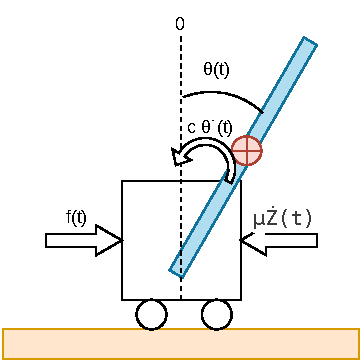
\includegraphics[scale=1]{sozai/1.pdf}
  \caption{ 倒立振子システム}
\end{figure}

\subsection{台車のパラメータ同定}

台車駆動系全体の運動方程式((4.1) 式の上式)のふるまいはパラメータ \(a\), \(b\) の値により決まる.
しかしながら,このパラメータ \(a\), \(b\) を直接的に測定することは困難である.
そこで,ここでは図 4.2 に示す台車駆動系の P 制御を行うことによって,未知パラメータ \(a\), \(b\) を
決定する方法について説明する.
まず,\( v(s) \) から \( z(s) \) への伝達関数 \( P(s) \) を求めると,

\[
  P(s) = \frac{b}{s(s + a)} \tag{4.2}
\]

である.台車を P コントローラ

\[
  v(t) = k_P \left( r(t) - z(t) \right) \tag{4.3}
\]

により制御したとき,台車位置の目標値 \( r(s) \) から制御量 \( z(s) \) への伝達関数 \( G(s) \) は

\[
  G(s) = \frac{P(s)k_P}{1 + P(s)k_P} = \frac{\omega_{n1}^2}{s^2 + 2\zeta_1 \omega_{n1} s + \omega_{n1}^2}, \tag{4.4}
\]

\[
  \omega_{n1} = \sqrt{\frac{b k_P}{a}}, \quad \zeta_1 = \frac{a}{2\omega_{n1}} = \frac{a}{2\sqrt{b k_P}}
\]
となる.ここで,目標値を

\[
  r(t) = 
  \begin{cases}
    0   & (t < 0)    \\
    z_c & (t \geq 0)
  \end{cases} \tag{4.5}
\]

とした 2 次遅れ要素のステップ応答は \(0 < \zeta_1 < 1\) のとき,

\[
  z(t) = z_c \left\{ 1 - e^{-\zeta_1 \omega_{n1} t}
  \left( \cos \omega_{d1} t + \frac{\zeta_1}{\sqrt{1 - \zeta_1^2}} \sin \omega_{d1} t \right) \right\} \tag{4.6}
\]
\[
  \omega_{d1} = \omega_{n1} \sqrt{1 - \zeta_1^2}
\]

であり,オーバーシュート \( A_{\text{max}} = z_{\text{max}} - z_c \) およびそのときの時間 \( T_{\text{peak}} \) は

\[
  A_{\text{max}} = z_c e^{-\zeta_1 \omega_{n1} T_{\text{peak}}}, \quad T_{\text{peak}} = \frac{\pi}{\omega_{d1}} \tag{4.7}
\]

となる.

したがって,実験データより \( T_{\text{peak}}, A_{\text{max}} \) を求めると,
(4.7) 式より \( \omega_{n1}, \zeta_1 \) が定まるから,未知パラメータ \( a, b \) が (4.4) 式を
逆算することにより計算できる.

\begin{figure}[h]
  \centering
  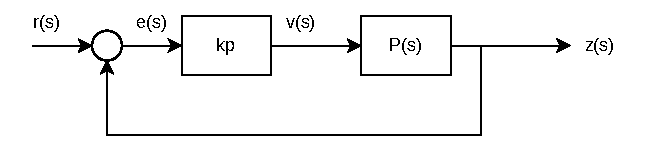
\includegraphics[scale=1]{sozai/2.pdf}
  \caption{台車駆動系のP制御}
\end{figure}

\subsection{振子のパラメータ同定}

台車を固定すると,(4.1) 式より振子の非線形モデルは
\[
  J\ddot{\theta}(t) = -c\dot{\theta}(t) - mgl\sin\theta(t) \quad (J = J_s + ml^2) \tag{4.8}
\]
となる.振子のパラメータ \( m, l, J_s \) である.振子の質量 \( m \) と重心位置 \( l \) は測定でき,
振子の慣性モーメントは床に対して下ろすことによりメジャーで測定できる.
しかしながら,慣性モーメント \( J_s \) を台車の動きに関連して測定することは難しい.
そこで,ここでは図 4.4 に示す振子の自由振動の測定データより \( J_s \) を決定する方法について説明する.

まず,振子の角度 \( \theta(t) \) を振子が床から下への大振幅を持つ \( \theta(t) \) について二乗近似し,
(4.8) 式を次のように書き換える:

\[
  J\ddot{\theta}(t) = -c\dot{\theta}(t) - mgl\sin\theta(t) \tag{4.9}
\]

と書き換える.このとき,\( \theta(t) \) に近づくと,振子のモデルは

\[
  J\ddot{\theta}(t) + 2\zeta_{2}\omega_{n2}\dot{\theta}(t) + \omega_{n2} \theta(t) = 0, \quad \omega_{n2} = \frac{mgl}{J}, \quad \zeta_2 = \frac{c}{2\sqrt{mglJ}} \tag{4.10}
\]

という 2 次の微分方程式で表されることがわかる.なお,振子に初期角度 \( \theta(0) = \theta_0 \)
(初期速度は0)を与えると (4.10) 式の解(自由振動解)は次のように表される:

\[
  \theta(t) = e^{-\zeta_{2}\omega_{n2}t} \left( \cos\omega_{d2}t + \frac{\zeta}{\sqrt{1-\zeta^2}} \sin \omega_d t \right), \quad \omega_d = \omega_n\sqrt{1-\zeta^2} \tag{4.11}
\]

となり,周期 \( T \),減衰率 \( \lambda \) は一定値

\[
  T = \frac{2\pi}{\omega_d2}, \quad \lambda = \frac{A_{k+1}}{A_k} = e^{-\zeta_{2}\omega_{n2} T} \tag{4.12}
\]

である.

以上より,実験データより振動周期 \( T = T_1 - T_2 \) および減衰率 
\( A_2/A_1 = A_3/A_2 \) を求めると,(4.12) 式をもとに \( \omega_n \) と \( \zeta \) 
が決定できるから,未知パラメータ \( c, J_s \) が (4.10) 式を逆算することにより計算できる.

\subsection{状態フィードバックによる倒立振子の安定化}

振子が \( \theta(t) = 0 \) の近傍であると仮定すると,

\[
  \cos \theta(t) \approx 1, \quad \sin \theta(t) \approx \theta(t)
\]

と近似できるから,(4.1) 式より近似線形化モデル

\[
  \begin{cases}
    \ddot{z}(t) = -a\dot{z}(t) + bv(t) \\
    ml\ddot{\theta}(t) + J\ddot{\theta}(t) = -c\dot{\theta}(t) + mgl\theta(t)
  \end{cases} \tag{4.13}
\]

が得られる.ここで,


\[
  \text{状態変数: }
  \begin{bmatrix}
    x_1(t) \\
    x_2(t) \\
    x_3(t) \\
    x_4(t)
  \end{bmatrix}
  =
  \begin{bmatrix}
    z(t)       \\
    \dot{z}(t) \\
    \theta(t)  \\
    \dot{\theta}(t)
  \end{bmatrix}
\]

\[ \text{操作量: } u(t) = v(t)  \]

とすると,(4.13) 式は状態方程式と呼ばれる1階の微分方程式

\[
  \dot{x}(t) = Ax(t) + Bu(t) \tag{4.14}
\]

で記述することができる.ただし,

\[
  A = \begin{bmatrix}
    0 & 1    & 0     & 0    \\
    0 & -a   & 0     & 0    \\
    0 & 0    & 0     & 1    \\
    0 & b/ml & mgl/J & -c/J
  \end{bmatrix}, \quad
  B = \begin{bmatrix}
    0 \\
    b \\
    0 \\
    mlb/J
  \end{bmatrix}
\]

である.

そこで,コントローラとして状態フィードバック

\[
  u(t) = Kx(t), \quad K = [k_1 \quad k_2 \quad k_3 \quad k_4] \tag{4.15}
\]

を用いて倒立振子を安定化することを考える.状態方程式 (4.14) 式と状態フィードバック (4.15) 式で
構成されるシステムは

\[
  \dot{x}(t) = Mx(t), \quad M = A + BK \tag{4.16}
\]

である.(4.16) 式の解は

\[
  x(t) = e^{Mt}x(0) \tag{4.17}
\]
となるので,システムの安定性は \( M \) の固有値により決まり,\( M \) の固有値の実部がすべて負であれば,
そのときに限りシステムは安定である.すなわち

\begin{itemize}
  \item 任意の初期値 \( x(0) \) に対して, \( t \to \infty \) で \( x(t) \to 0 \)
\end{itemize}

となる(注4).したがって,\( M \) の固有値の実部がすべて負となるように状態フィードバックゲイン \( K \) 
を決定すれば,振子は倒立する(倒立振子は安定化される).

本実験では,アッカーマンのアルゴリズムにより \( M \) の固有値が指定した値 \( p_i \ (i=1,2,3,4) \) 
となるように状態フィードバックゲイン \( K \) を定める.ただし,\( \text{Re}[p_i] < 0 \) となるように
\( p_i \) を決める.

\section{実験 2}
\subsection{実験 2-1: 台車のパラメータ同定}
\subsubsection{実験方法}

\begin{enumerate}
  \item カレントディレクトリを D:\textbackslash experiment\_5S\textbackslash group01\textbackslash cart\_ident とし,配布する Simulink モデル "ex\_cart\_ident.slx"(図 A.7)を開く."ex\_cart\_ident.slx" は目標値 \( z_c \),比例ゲイン \( k_p \) が "kP" に設定されている.つぎに,Subsystem (Inverted Pendulum) 内の Simulink ブロックを
        \begin{itemize}
          \item Gain (polarity): ゲインに "1" もしくは "-1" を入力(3.4 節を参照)
          \item Gain (count to rad): ゲインを 1 カウントあたりの振子角度変位 \( \alpha \) に変更(3.2 節を参照)
          \item Gain (count to meter): ゲインを 1 カウントあたりの台車位置変位 \( \beta \) に変更(3.3 節を参照)
        \end{itemize}
  \item (振子を台車に取り付けたまま)レールの中央付近に台車を配置する.つぎに,
        \begin{itemize}
          \item 指令電圧 \( v(t) \) が制限値 ±10 [V] を超えない
          \item オーバーシュートを生じる
          \item 台車がレールを超えない (0 < \( z_c \leq 0.2 \) の範囲で設定)
        \end{itemize}
        という制約を満足する比例ゲイン \( k_p > 0 \),目標値 \( z_c > 0 \) を 3 種類選ぶ.1 種類目の \( k_p \),\( z_c \) をコマンドウィンドウで
        \begin{tcolorbox}[colback=gray!5!white,colframe=gray!75!black]
          \begin{lstlisting}
    >> kP = ***; zc = ***;
    \end{lstlisting}
        \end{tcolorbox}
        と入力("***" には各項で考えた正数)した後,ビルドしてエラーがないことを確認する.Simulink モデルの実行を開始し,オーバーシュートが生じるかどうかを確認する(Scope をダブルクリックして開いておくと,リアルタイムで台車位置を観測できる).実験終了後,コマンドウィンドウで
        \begin{tcolorbox}[colback=gray!5!white,colframe=gray!75!black]
          \begin{lstlisting}
    >> save cart_data t z v kP zc
    \end{lstlisting}
        \end{tcolorbox}
        と入力し,実験データを "cart\_data.mat" という名前の mat ファイルに保存する.同様に,以下の実験を行う.
        \begin{itemize}
          \item 2 種類目の \( k_p \),\( z_c \) を用いて実験を行い,実験データを "cart\_data2.mat" という名前の mat ファイルに保存する
          \item 3 種類目の \( k_p \),\( z_c \) を用いて実験を行い,実験データを "cart\_data3.mat" という名前の mat ファイルに保存する
        \end{itemize}
  \item 配布する M ファイル "plot\_cart.m" を実行することにより,以下のことを行う.
        \begin{enumerate}
          \item 1 種類目の実験データからオーバーシュート \( A_{\text{max}} \),行き過ぎ時間 \( T_{\text{peak}} \) を抽出する.\\
                表 5.1 に記入
          \item (4.7) 式より固有角周波数 \( \omega_{n1} \),減衰係数 \( \zeta_1 \) をオーバーシュート \( A_{\text{max}} \),行き過ぎ時間 \( T_{\text{peak}} \) により表す.
                \[
                  \omega_{n1} = {\large\textbf{        }} , \quad \zeta_1 = {\large\textbf{        }}
                \]
                この関係を利用し,実験により得られた \( A_{\text{max}}, T_{\text{peak}} \) から \( \omega_{n1}, \zeta_1 \) を定める.\\
          \item 2 種類目の \( z_c \), \( k_p \): M ファイル "plot\_cart2.m" を実行し,抽出された \( A_{\text{max}}, T_{\text{peak}} \) の値,定められた \( \omega_{n1}, \zeta_1 \) の値を表に記入
          \item 3 種類目の \( z_c \), \( k_p \): M ファイル "plot\_cart3.m" を実行し,抽出された \( A_{\text{max}}, T_{\text{peak}} \) の値,定められた \( \omega_{n1}, \zeta_1 \) の値を表に記入
        \end{enumerate}
        
  \item 配布する M ファイル "idcart.m" を実行することにより,以下のことを行う.
        \begin{enumerate}
          \item 得られた \( \omega_{n1}, \zeta_1 \) をコマンドウィンドウに入力することで,実験結果と同定された値を用いたシミュレーション結果を描画し,両者がほぼ一致していることを確認する.
          \item (4.4) 式より未知パラメータ \( a, b \) を \( \omega_{n1}, \zeta_1 \) により表す.
                \[
                  a = {\large\textbf{        }} , \quad b ={\large\textbf{        }}
                \]
                この関係を利用して未知パラメータ \( a, b \) の値を定める.\\
          \item 2 種類目の \( z_c \), \( k_p \): M ファイル "idcart2.m" を実行し,定められた \( a, b \) の値を表に記入
          \item 3 種類目の \( z_c \), \( k_p \): M ファイル "idcart3.m" を実行し,定められた \( a, b \) の値を表に記入
        \end{enumerate}
\end{enumerate}



\subsubsection{実験結果}

\paragraph{(a) 1 種類目の実験データ}
\begin{itemize}
  \item \( k_p \), \( z_c \) を \\
        \( k_p = {\large\textbf{ 100  }}  , \quad z_c = {\large\textbf{  0.1  }} \)
\end{itemize}

と選び,図 A.7 の Simulink モデルを実行したときに得られた実験データから抽出された \( A_{\text{max}}, T_{\text{peak}} \) の値を表 5.1 に示す.
\begin{itemize}
  \item 実験方法 (3) の (ii) で示した関係式により定められた \( \omega_{n1}, \zeta_1 \) の値を表 5.2 に,実験結果と同定された値を用いたシミュレーション結果を示す.
  \item 実験方法 (4) の (ii) で示した関係式により定められた \( a, b \) の値を表 5.3 に示す.
\end{itemize}

\begin{table}[h]
  \centering
  \caption{台車のステップ応答における \( A_{\text{max}}, T_{\text{peak}} \)}
  \label{tab:exp_data_1}
  \begin{tabular}{|c|c|}
    \hline
    オーバーシュート \( A_{\text{max}} \) [m] & 行き過ぎ時間 \( T_{\text{peak}} \) [s] \\
    \hline
    \( 2.71e^{-02}\)                          & \( 3.20e^{-01}\)                       \\
    \hline
  \end{tabular}
\end{table}

\begin{table}[h]
  \centering
  \caption{台車のステップ応答における \( \omega_{n1}, \zeta_1 \)}
  \label{tab:exp_data_2}
  \begin{tabular}{|c|c|}
    \hline
    固有角周波数 \( \omega_{n1} \) & 減衰係数 \( \zeta_1 \) \\
    \hline
    \( 1.06e^{+01}\)               & \( 3.84e^{-01}\)       \\
    \hline
  \end{tabular}
\end{table}

\begin{table}[h]
  \centering
  \caption{台車駆動系のパラメータ}
  \label{tab:drive_system_parameters}
  \begin{tabular}{|c|c|}
    \hline
    a & \( 8.16e^{+00}\) \\
    \hline
    b & \( 1.13e^{+00}\) \\
    \hline
  \end{tabular}
\end{table}

\begin{figure}[h]
  \centering
  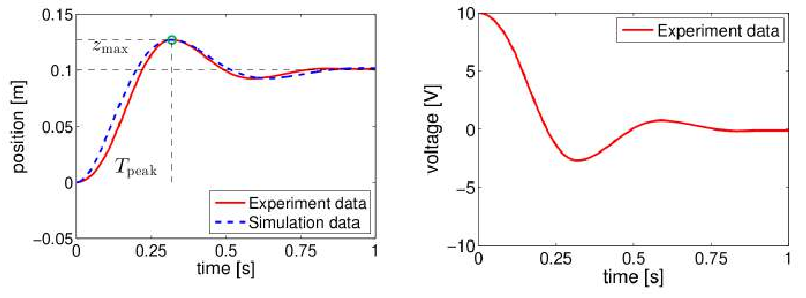
\includegraphics[scale=1]{sozai/51.pdf}
  \caption{台車のP制御の実験結果とシュミレーション結果}
\end{figure}

\paragraph{(b) 2 種類目の実験データ}
\begin{itemize}
  \item \( k_p \), \( z_c \) を \\
        \( k_p = {\large\textbf{  1500   }} , \quad z_c = {\large\textbf{ 0.1   }}\)
\end{itemize}

として (a) と同様の実験を行い,結果を表 5.4,表 5.5,図 5.2 および表 5.6 に示す.

\begin{table}[h]
  \centering
  \caption{台車のステップ応答における \( A_{\text{max}}, T_{\text{peak}} \)}
  \label{tab:step_response_1}
  \begin{tabular}{|c|c|}
    \hline
    オーバーシュート \( A_{\text{max}} \) [m] & 行き過ぎ時間 \( T_{\text{peak}} \) [s] \\
    \hline
    \( 5.66e^{-02}\)                          & \( 3.17e^{-01}\)                       \\
    \hline
  \end{tabular}
\end{table}

\begin{table}[h]
  \centering
  \caption{台車のステップ応答における \( \omega_{n1}, \zeta_1 \)}
  \label{tab:step_response_2}
  \begin{tabular}{|c|c|}
    \hline
    固有角周波数 \( \omega_{n1} \) & 減衰係数 \( \zeta_1 \) \\
    \hline
    \(1.01e^{+01}\)                & \( 1.78e^{-01}\)       \\
    \hline
  \end{tabular}
\end{table}

\begin{table}[h]
  \centering
  \caption{台車駆動系のパラメータ}
  \label{tab:drive_system_parameters_2}
  \begin{tabular}{|c|c|}
    \hline
    a & \(3.59e^{+00}\)  \\
    \hline
    b & \( 6.76e^{-02}\) \\
    \hline
  \end{tabular}
\end{table}

\begin{figure}[h]
  \centering
  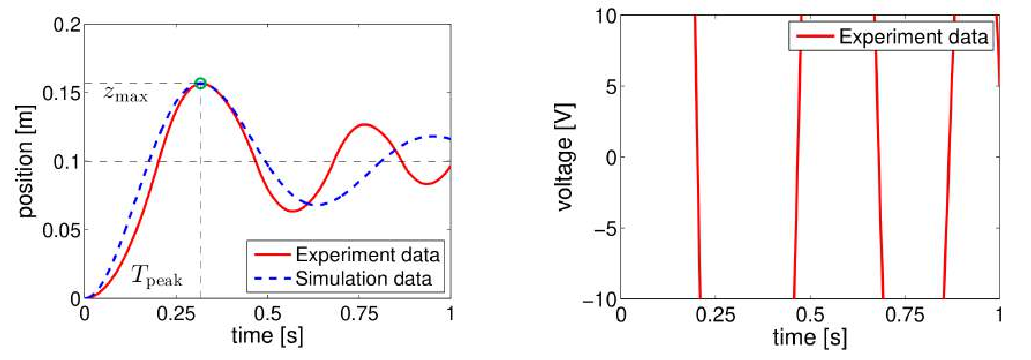
\includegraphics[scale=1]{sozai/52.pdf}
  \caption{台車のP制御の実験結果とシュミレーション結果}
\end{figure}

\paragraph{(c) 3 種類目の実験データ}
\begin{itemize}
  \item \( k_p \), \( z_c \) を \\
        \( k_p ={\large\textbf{ 100   }} , \quad z_c ={\large\textbf{  0.2    }} \)
\end{itemize}

として (a) と同様の実験を行い,結果を表 5.7,表 5.8,図 5.3 および表 5.9 に示す.

\begin{table}[h]
  \centering
  \caption{台車のステップ応答における \( A_{\text{max}}, T_{\text{peak}} \)}
  \label{tab:step_response_3}
  \begin{tabular}{|c|c|}
    \hline
    オーバーシュート \( A_{\text{max}} \) [m] & 行き過ぎ時間 \( T_{\text{peak}} \) [s] \\
    \hline
    \( 4.36e^{-02}\)                          & \( 3.92e^{-02}\)                       \\
    \hline
  \end{tabular}
\end{table}

\begin{table}[h]
  \centering
  \caption{台車のステップ応答における \( \omega_{n1}, \zeta_1 \)}
  \label{tab:step_response_4}
  \begin{tabular}{|c|c|}
    \hline
    固有角周波数 \( \omega_{n1} \) & 減衰係数 \( \zeta_1 \) \\
    \hline
    \( 8.91e^{+00}\)               & \( 4.37e^{-01}\)       \\
    \hline
  \end{tabular}
\end{table}

\begin{table}[h]
  \centering
  \caption{台車駆動系のパラメータ}
  \label{tab:drive_system_parameters_3}
  \begin{tabular}{|c|c|}
    \hline
    a & \( 7.78e^{+00}\) \\
    \hline
    b & \( 7.93e^{-01}\) \\
    \hline
  \end{tabular}
\end{table}

\begin{figure}[h]
  \centering
  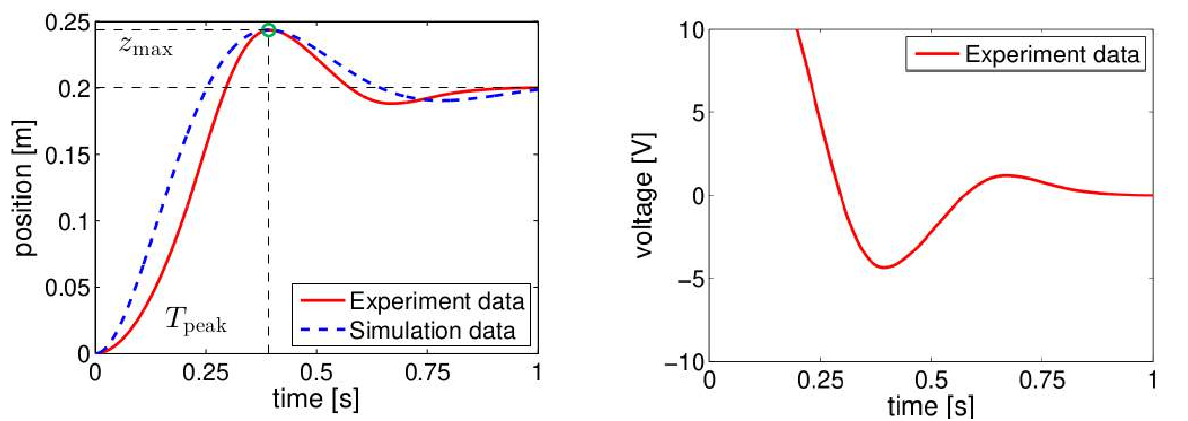
\includegraphics[scale=0.7]{sozai/53.pdf}
  \caption{台車のP制御の実験結果とシュミレーション結果}
\end{figure}

\newpage

\subsubsection{実験考察}
3種類のうち2種類は制約を超えてしまっている.
これは,式(3.4)\(v(t) = k_P \left( r(t) - z(t) \right)\)のため
1種類目は初期出力は10Vであると考えられ
制約は守られている.しかし,2種類目,3種類目に関しては計算値がそれぞれ最大150V,20Vとなっており
守れていない.図5.1より初期値が10Vであることからも正しいことがわかる.
実験結果とシュミレーション結果のズレには振子の揺れが関係していると考えられる.
動いた際に台車本体に振動が伝わり,台車の移動に影響があったのではないかと考える.
他には,モーターの加速時間と摩擦が関係していると考えられる.
モーター初期起動時に理論値に比べ速度が上がらなかったことも原因の一つであると考えられる.



\subsection{実験 2-2: 振子のパラメータ同定}
\subsubsection{実験方法}

振子を取り外して,その質量 \( m \) をはかりで測定すると \( m = 2.30 \times 10^{-1} \) [kg] であった.また振子をひもでつるして重心位置を調べると \( l = 3.05 \times 10^{-1} \) [m] であった.

\begin{enumerate}
  \item カレントディレクトリを D:\textbackslash experiment\_5S\textbackslash group01\textbackslash pend\_ident に変更する.Simulink モデル "ex\_pend\_ident.slx"(図 A.8)を開き,5.1 節と同様に Subsystem (Inverted Pendulum) 内の Simulink ブロック(三つの Gain)の設定を変更した後,上書き保存する.
        また,ビルドしてエラーがないことを確認した後,
        "ex\_pend\_ident.pdf","ex\_pend\_ident.bmp" 
        という名前の pdf ファイル,bmp ファイルを生成し,
        pdf ファイルはデスクトップ上の "bcpdfcrop-multi.bat" 
        により余白を取り除く.
        
  \item 台車に振子を取り付け,振子を振ったときに台車が動かないように,
        手でしっかりと台車を固定する.
        また,振子をぶら下がった状態で静止させる.
        
  \item ここで,Simulink モデルの実行を開始し,10 秒以内に振子を 90 [deg](水平)付近まで傾けて静かに手を離し,
        振子角度 \( \theta(t) \) を計測する.
        30 秒で実行は終了するので,コマンドウィンドウで
        \begin{tcolorbox}[colback=gray!5!white,colframe=gray!75!black]
          \begin{lstlisting}
            >> save pend_data t phi
            \end{lstlisting}
        \end{tcolorbox}
        と入力し,実験データを "pend\_data.mat" という名前の mat ファイルに保存する.同様に,Simulink モデルの実行を開始し,10 秒以内に振子を 30 [deg] 付近まで傾けて静かに手をはなし,30 秒で実行は終了するので,実験データを "pend\_data2.mat" という名前の mat ファイルに保存する.
        
        t.pdf","ex\_cart\_ident.bmp" という名前の pdf ファイル,bmp ファイルを生成し,pdf ファイルはデスクトップ上の "bcpdfcrop-multi.bat" により余白を取り除く.
\end{enumerate}

\subsubsection{実験結果}
\subsection*{(a) 初期角度を約 90 deg とした場合}

図 A.8 の Simulink モデルを実行し,得られた実験データから抽出された周期 
\( T_1, \cdots, T_{10} \) と減衰率 \( \lambda_1, \cdots, \lambda_{10} \) 
およびこれらの平均値 \( T, \lambda \) を表 5.10 に,グラフ化したものを図 5.4 に示す.
実験方法 (3) の (ii) で示した関係式により定められた \( \omega_{n2}, \zeta_2 \) の値を表 5.11 に,
実験結果と間定された値を用いたシミュレーション結果を図 5.5 に示す.また,実験方法 (3) の (iii) 
で示した関係式により定められた \( c, J_g \) の値を表 5.12 に示す.

\begin{table}[h]
  \centering
  \caption{振子の振動周期 \( T \) と減衰率 \( \lambda \)}
  \label{tab:振子の振動周期と減衰率}
  \begin{tabular}{|c|c|}
    \hline
    振動周期 [s]                        & 減衰率                                     \\
    \hline
    \( T_1 = 1.4565 \times 10^{0} \)    & \( \lambda_1 = 9.6028 \times 10^{-1} \)    \\
    \( T_2 = 1.4435 \times 10^{0} \)    & \( \lambda_2 = 9.6229 \times 10^{-1} \)    \\
    \( T_3 = 1.4330 \times 10^{0} \)    & \( \lambda_3 = 9.6334 \times 10^{-1} \)    \\
    \( T_4 = 1.4240 \times 10^{0} \)    & \( \lambda_4 = 9.6588 \times 10^{-1} \)    \\
    \( T_5 = 1.4150 \times 10^{0} \)    & \( \lambda_5 = 9.6739 \times 10^{-1} \)    \\
    \( T_6 = 1.4075 \times 10^{0} \)    & \( \lambda_6 = 9.6770 \times 10^{-1} \)    \\
    \( T_7 = 1.4000 \times 10^{0} \)    & \( \lambda_7 = 9.6807 \times 10^{-1} \)    \\
    \( T_8 = 1.3950 \times 10^{0} \)    & \( \lambda_8 = 9.7001 \times 10^{-1} \)    \\
    \( T_9 = 1.3895 \times 10^{0} \)    & \( \lambda_9 = 9.7063 \times 10^{-1} \)    \\
    \( T_{10} = 1.3850 \times 10^{0} \) & \( \lambda_{10} = 9.7293 \times 10^{-1} \) \\
    \hline
    平均 \( T = 1.4149 \times 10^{0} \) & 平均 \( \lambda = 9.6685 \times 10^{-1} \) \\
    \hline
  \end{tabular}
\end{table}

\begin{table}[h]
  \centering
  \begin{minipage}{0.45\linewidth}
    \centering
    \caption{振子の自由振動における $\omega_{n2}, \zeta_2$}
    \begin{tabular}{|c|c|}
      \hline
      固有角周波数 $\omega_{n2}$ & 4.4408e+00 \\
      \hline
      減衰係数 $\zeta_2$         & 5.3650e-03 \\
      \hline
    \end{tabular}
  \end{minipage}
  \hfill
  \begin{minipage}{0.45\linewidth}
    \centering
    \caption{振子のパラメータ}
    \begin{tabular}{|c|c|}
      \hline
      $J_g$ [kg$\cdot$m$^2$] & 1.35e-02 \\
      \hline
      $c$ [kg$\cdot$m$^2$/s] & 1.66e-03 \\
      \hline
    \end{tabular}
  \end{minipage}
\end{table}

\begin{figure}[h]
  \centering
  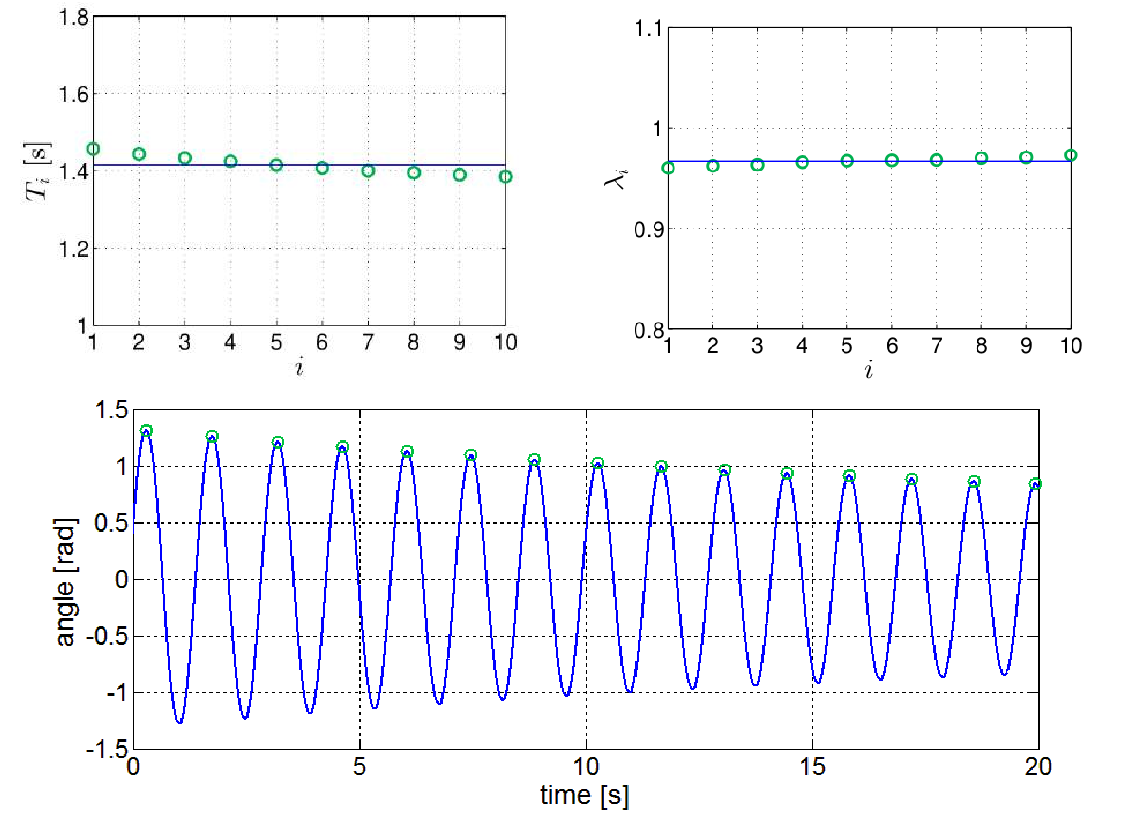
\includegraphics[scale=0.7]{sozai/6.pdf}
  \caption{振子の自由振動の実験結果と振動周期,減衰率}
\end{figure}

\begin{figure}[h]
  \centering
  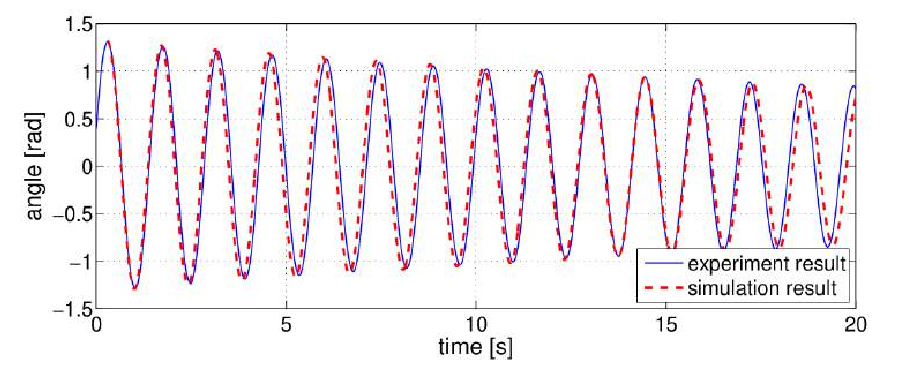
\includegraphics[scale=0.7]{sozai/7.pdf}
  \caption{振子の自由振動の実験結果と線形シュミレーション結果との比較}
\end{figure}

\subsubsection*{(b) 初期角度を約 30 deg とした場合}

初期角度を約 30 deg として (a) と同様の実験を行い,結果を表 5.13,図 5.6,表 5.14 および表 5.15 
に示す.

\begin{table}[h]
  \centering
  \caption{振子の振動周期 $T$ と減衰率 $\lambda$}
  \begin{tabular}{|c|c|}
    \hline
    振動周期 [s]          & 減衰率                      \\
    \hline
    $T_1 = 1.3400e+00$    & $\lambda_1 = 9.8272e-01$    \\
    \hline
    $T_2 = 1.3365e+00$    & $\lambda_2 = 9.7990e-01$    \\
    \hline
    $T_3 = 1.3360e+00$    & $\lambda_3 = 9.8205e-01$    \\
    \hline
    $T_4 = 1.3355e+00$    & $\lambda_4 = 9.8172e-01$    \\
    \hline
    $T_5 = 1.3335e+00$    & $\lambda_5 = 9.8138e-01$    \\
    \hline
    $T_6 = 1.3325e+00$    & $\lambda_6 = 9.8374e-01$    \\
    \hline
    $T_7 = 1.3320e+00$    & $\lambda_7 = 9.8072e-01$    \\
    \hline
    $T_8 = 1.3315e+00$    & $\lambda_8 = 9.8315e-01$    \\
    \hline
    $T_9 = 1.3300e+00$    & $\lambda_9 = 9.8286e-01$    \\
    \hline
    $T_{10} = 1.3300e+00$ & $\lambda_{10} = 9.8547e-01$ \\
    \hline
    平均 $T = 1.3337e+00$ & 平均 $\lambda = 9.8186e-01$ \\
    \hline
  \end{tabular}
\end{table}

\begin{table}[h]
  \centering
  \begin{minipage}{0.45\linewidth}
    \centering
    \caption{振子の自由振動における $\omega_{n2}$, $\zeta_2$}
    \begin{tabular}{|c|c|}
      \hline
      固有角周波数 $\omega_{n2}$ & 減衰係数 $\zeta_2$ \\
      \hline
      $4.7109e+00$               & $2.8310e-03$       \\
      \hline
    \end{tabular}
  \end{minipage}%
  \hfill
  \begin{minipage}{0.45\linewidth}
    \centering
    \caption{振子のパラメータ}
    \begin{tabular}{|c|c|}
      \hline
      $J_g$ [kg$\cdot$m$^2$] & $c$ [kg$\cdot$m$^2$/s] \\
      \hline
      $9.61e-03$             & $8.27e-04$             \\
      \hline
    \end{tabular}
  \end{minipage}
\end{table}

\newpage

\begin{figure}[H]
  \centering
  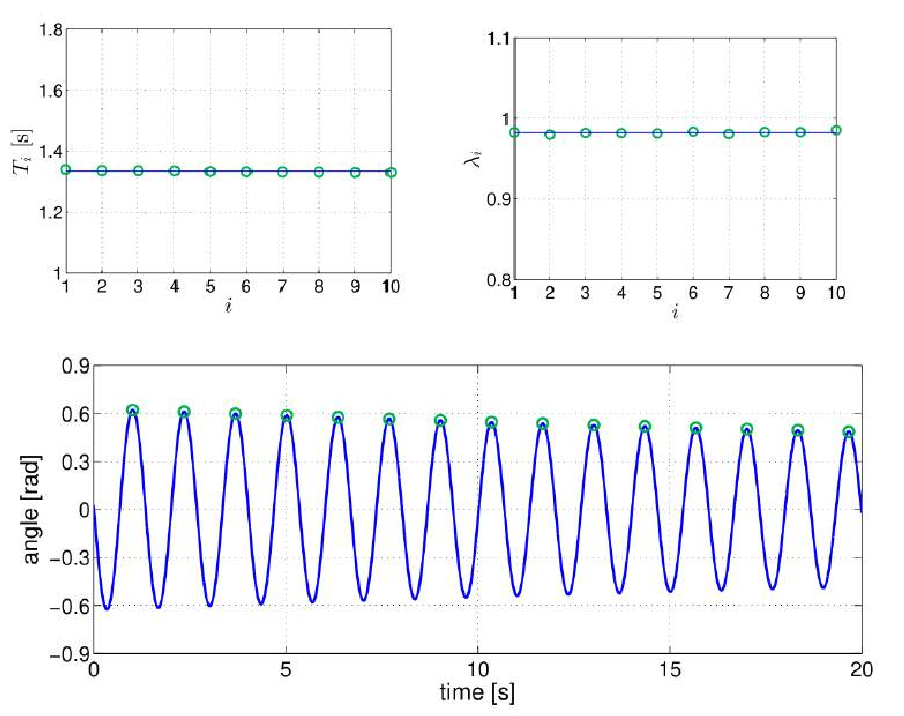
\includegraphics[scale=0.7]{sozai/8.pdf}
  \caption{振子の自由振動の実験結果と振動周期,減衰率}
\end{figure}

\begin{figure}[H]
  \centering
  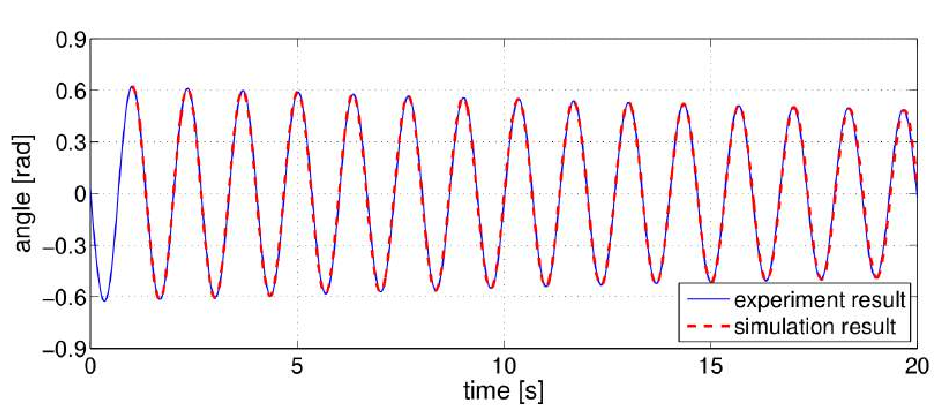
\includegraphics[scale=0.7]{sozai/9.pdf}
  \caption{振子の自由振動の実験結果と線形シュミレーション結果との比較}
\end{figure}


\subsubsection{実験考察}

振子の減衰率や周期が一定ではないことが確認された。
実験環境では、振子の動きに軸受けの摩擦や空気抵抗が影響を与えるため、
これらの要因が振動に不規則な影響を及ぼし、結果として減衰率や周期にばらつきが生じたと考えられる。
これらの外部要因が振子の運動に微妙な変化をもたらし、振動の周期や減衰率が一貫しない原因となっている。

倒立振子の初期角度が大きい場合、線形シミュレーションと実験結果の間にズレが発生する。
このズレは、振子の角度が大きくなると、角度の近似が適用できなくなることに起因する。
具体的には、線形モデルでは以下の近似が用いられる。

\[
  \cos \theta(t) \approx 1, \quad \sin \theta(t) \approx \theta(t)
\]

しかし、角度 \( \theta(t) \) が大きくなると、この近似が成立しなくなり、
実際の挙動とシミュレーションの結果にズレが生じる。近似条件が満たされなくなるため、
線形モデルでは大きな角度での正確なシミュレーションが困難となる。
このため、初期角度が大きい場合に線形シミュレーションと実験結果の間に誤差が生じると考えられる。


\subsection{実験 2-3: 状態フィードバックによる安定化}
\subsubsection{実験方法}

\paragraph{実験 2-3a}
\begin{enumerate}
  \item カレントディレクトリを D:\textbackslash experiment\_5S\textbackslash group01\textbackslash stable に移動する.配布する M ファイル "ip\_design.m" を実行し,メニューにしたがってパラメータ同定実験で得られたパラメータおよび指定する \( M = A + BK \) の固有値を入力する.ただし,\( M \) の固有値は表 5.16 のように指定する.このとき,極配置法(MATLAB 関数 "acker")により状態フィードバックゲイン \( K = [k_1, k_2, k_3, k_4] \) が求められる.\\
        表 5.16 に記入
        
  \item D:\textbackslash experiment\_5S\textbackslash group01\textbackslash stable にある Simulink モデル "ex\_stable.slx" (図 A.9) を開き,5.1 節と同様に Subsystem (Inverted Pendulum) 内の Simulink ブロック(三つの Gain)の設定を変更し,上書き保存する.また,"ex\_stable.pdf","ex\_stable.bmp" という名前の pdf ファイル,bmp ファイルを生成し,pdf ファイルはデスクトップ上の "bcpdfcrop-multi.bat" により余白を取り除く.つぎに,Simulink モデル "ex\_stable.slx" をビルドしてエラーが生じないことを確認する.そして,
        
        \begin{tcolorbox}[colback=gray!5!white,colframe=gray!75!black]
          \begin{lstlisting}
    Manual Switch が Constant 側になっている(指令電流を u(t) = 0 [V] とすることになるので,台車は静止する)
    \end{lstlisting}
        \end{tcolorbox}
        
        振子がぶら下がった状態で静止していることを確認する.
        
  \item Simulink モデルの実行を開始する.実行開始後,振子を手で静かに倒立状態にし,Manual Switch をダブルクリックして Gain 側にする.状態フィードバックを介して倒立状態が維持され,振子が倒立状態になったことを確認する.実験終了後,コマンドウィンドウで
        
        \begin{tcolorbox}[colback=gray!5!white,colframe=gray!75!black]
          \begin{lstlisting}
    >> save stable_data1 t x u dz dtheta
    \end{lstlisting}
        \end{tcolorbox}
        
        と入力し,実験データを "stable\_data1.mat" という名前の mat ファイルに保存する.
        
  \item M の固有値 \( p_i \) を表 5.17 のように指定し,同様の実験を行う.また,振子の先を軽くつついたとき,表 5.16 のように指定した場合との差異を調べる.また,必要に応じて
        
        \begin{tcolorbox}[colback=gray!5!white,colframe=gray!75!black]
          \begin{lstlisting}
    >> save stable_data2 t x u dz dtheta
    \end{lstlisting}
        \end{tcolorbox}
        
        と入力し,実験データを "stable\_data2.mat" という名前の mat ファイルに保存する.
\end{enumerate}

\paragraph{実験 2-3b}
実験 2-3a では,振子が真下で静止している状態で Simulink モデル 
"ex\_stable.slx" の実行を開始し,振子が真上にあるときの角度を
正確に 0 [deg] として検出するようにしている
(\textbf{実験 1-1c を参照}).

実験 2-3b では,あえて振子が真下から少しだけずれている状態で
Simulink モデル "ex\_stable.slx" の実行を開始し
,図 5.8 のように振子の角度検出にずれがあるときのふるまいを調べる.

\subsubsection{実験結果}

\paragraph{実験 2-3a}
設計されたコントローラのゲイン \( K \) を表 5.16 に示す.また,図 A.8 の Simulink モデルを実行して安定化を実現したときの設計例 1 と設計例 2 のふるまいの違いを表 5.18 に示す.

\begin{table}[h]
  \centering
  \caption{設計例 1}
  \label{tab:design_example_1}
  \begin{tabular}{|c|c|}
    \hline
    \( M \) の固有値 & 設計された \( K \)  \\
    \hline
    \( p_1 = -5 \)   & \( k_1 \) 2.32e+01  \\
    \( p_2 = -5 \)   & \( k_2 \) 2.55e+01  \\
    \( p_3 = -5 \)   & \( k_3 \)  7.33e+01 \\
    \( p_4 = -5 \)   & \( k_4 \)  1.55e+01 \\
    \hline
  \end{tabular}
\end{table}

\begin{table}[h]
  \centering
  \caption{設計例 2}
  \label{tab:design_example_2}
  \begin{tabular}{|c|c|}
    \hline
    \( M \) の固有値    & 設計された \( K \)  \\
    \hline
    \( p_1 = -5 + 5j \) & \( k_1 \)  9.29e+01 \\
    \( p_2 = -5 - 5j \) & \( k_2 \) 4.42e+01  \\
    \( p_3 = -5 + 5j \) & \( k_3 \)  1.22e+02 \\
    \( p_4 = -5 - 5j \) & \( k_4 \)  2.37e+01 \\
    \hline
  \end{tabular}
\end{table}

\begin{table}[h]
  \centering
  \caption{安定化の様子}
  \label{tab:stabilization_observation}
  \begin{tabular}{|c|c|c|c|c|}
    \hline
    設計例   & 反応の速さ                    & 安定度                        & 収束の速さ                        & チャタリングの影響              \\
    \hline
    設計例 1 & {\large\textbf{  遅い  }} & {\large\textbf{  高い  }} & {\large\textbf{   同じ   }} & {\large\textbf{  小さい  }} \\
    設計例 2 & {\large\textbf{  早い  }} & {\large\textbf{  低い  }} & {\large\textbf{   同じ   }} & {\large\textbf{  大きい  }} \\
    \hline
  \end{tabular}
\end{table}

\paragraph{実験 2-3b}
台車および振子の静止位置がどのようになったのかを,記述すること.

\subsection{実験結果}
少し初期位置よりずれた.

\subsection{実験考察}
コントローラの挙動は,固有値 \( p_i = a_i + jb_i \) の実部 \( a_i \) と虚部 \( b_i \) 
の大きさに密接に関連している.
固有値の実部は,システムの減衰特性に影響を与え,
負の実部が大きいほどシステムは速く減衰して安定する.
一方,虚部 \( b_i \) は振動の周波数に影響を与え,振動の速さや周期に関係する.

\begin{itemize}
  \item \textbf{実部が大きい場合}: 速やかに減衰し,振動が抑えられるため,システムは早く安定する.
  \item \textbf{虚部が大きい場合}: システムは高周波数で振動しやすくなる.
\end{itemize}

振子の基準が正確に真上に設定されていない場合,
システムはバランスをとるために台車がずれた位置で静止することになる.
これは,振子が不安定な位置から少しずれた状態で止まってしまうことによって,
台車がその位置でバランスを取ろうとするためだと考えられる.

\section{検討課題}

\subsection*{課題1}
ロータリエンコーダについて,以下の事項を説明せよ.
\begin{itemize}
  \item インクリメンタル型のカウントの数え方には,1逓倍,2逓倍,4逓倍がある.図を用いて各逓倍を説明せよ.
  \item アブソリュート型のスリットの配置図を示せ(3ビットの場合).また,インクリメンタル型,アブソリュート型の特徴について説明せよ.
\end{itemize}

アブソリュート型エンコーダは,各位置に固有のコードを持つことによって,絶対的な位置を検出することができる.
これにより,電源が切れたり,システムが再起動した場合でも,正確な位置情報を保持することができる.
インクリメンタル型エンコーダは,相対位置を基準位置からの変位として検出する.
このタイプのエンコーダは,電源が切れた場合や再起動した場合には,基準位置に戻す必要があるが,
構造が比較的簡単であり,コストも安価である.

\begin{figure}[h]
  \centering
  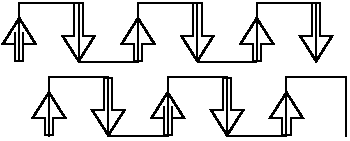
\includegraphics[scale=0.8]{sozai/11.pdf}
  \caption{カウントの数え方}
\end{figure}

図6.1に4逓倍のときの数え方を示す.4逓倍時はすべての立ち上がり及びたち下がりを見ることにより精度を増加させる.
1逓倍のときは一つに立ち上がり,2逓倍ではA,Bそれぞれの立ち上がりを見る.

以下の図\ref{fig:abs_encoder}に,アブソリュート型エンコーダの3ビットの場合のスリット配置を示す.
\begin{figure}[h]
  \centering
  
\includegraphics[scale=0.5]{sozai/10.pdf}
  \caption{アブソリュート型エンコーダのスリット配置(3ビット)}
  \label{fig:abs_encoder}
\end{figure}



\subsection*{課題2}
本実験装置では,リニアホールの電力増幅器が用いられているが,実際の現場では,PWM方式が用いられることが多い.PWM方式の電力増幅について調べよ.

PWM方式の電力増幅器には高効率であり,低発熱である.
トランジスタがオンまたはオフの状態のみで動作するため,エネルギー損失が少ない.
また,トランジスタが線形動作しないため,発熱が少なく調整できる点が利点である.


\subsection*{課題3}
質量$m$で長さ$l$の均質な直線棒の重心(中心)まわりの慣性モーメントが $J_g = \frac{1}{3}ml^2$ となることを示せ.また,$m = 2.30 \times 10^{-1} \, \mathrm{kg}, l = 3.05 \times 10^{-1} \, \mathrm{m}$ としたときの $J_g = \frac{1}{3}ml^2$ と,5.2節の実験で得られた $J_g$ の値を比較し,両者に差異が生じている主な要因を述べよ.


質量 \(m\) で長さ \(l\) の均質な直線棒の重心周りの慣性モーメントが \(J_g = \frac{1}{3}ml^2\) となることを示す.

直線棒の密度は \(\rho = \frac{m}{2l}\) によって求めることができるので,重心周りの慣性モーメントは次のように表される:
\[
  J_g = \int_{-l}^{l} x^2 \rho \, dx = \frac{m}{2l} \int_{-l}^{l} x^2 \, dx
\]
ここで,\(x^2\) は偶関数であるため,積分の結果は次のように求まる:
\[
  J_g = \frac{m}{2l} \int_{-l}^{l} x^2 \, dx = \frac{m}{2l} \cdot \frac{2}{3} l^3 = \frac{1}{3} ml^2
\]

実験条件として,質量 \(m = 2.30 \times 10^{-1}\) [kg],長さ \(l = 3.05 \times 10^{-1}\) [m] としたとき,理論的に求まる慣性モーメントの値を計算すると:
\[
  J_g = \frac{1}{3}ml^2 = \frac{1}{3} \cdot 2.30 \times 10^{-1} \cdot (3.05 \times 10^{-1})^2 = 7.1319 \times 10^{-3} \, \text{kg} \cdot \text{m}^2
\]
となる.

実験で得られた値 \(J_g\) は,理論値と比較して若干大きい値が得られた.
実世界における空気抵抗などの影響があると考えられる.

\subsection*{課題4}
(4.12) 式より $\omega_{n2}, \zeta_2$ を $A_{\max}, T_{\text{peak}}$ により表せ.
以下の式で $\omega_{n2}$ と $\zeta_2$ が表される:
\[
  \zeta_1 = \frac{1}{\sqrt{\pi^2 + \left( \ln \frac{z_c}{A_{\max}} \right)^2}} \ln \frac{z_c}{A_{\max}}
\]
\[
  \omega_{n2} = \frac{\sqrt{\pi^2 + \left( \ln \frac{z_c}{A_{\max}} \right)^2}}{T_{\text{peak}}}
\]

\subsection*{課題5}
(4.12) 式に $\omega_{n2}, \zeta_2$ を $T, \lambda$ により表せ.

周期 \(T\) の式より

\[
  T = \frac{\pi}{\omega_{d2}} = \frac{\pi}{\omega_{n2} \sqrt{1 - \zeta_2^2}} \tag{1}
\]

この式を \(\omega_{n2}\) について解くと,

\[
  \omega_{n2} = \frac{\pi}{T \sqrt{1 - \zeta_2^2}} \tag{2}
\]

次に、式 (4.12) より、減衰率 \(\lambda\) の式を用い,
\[
  \lambda = e^{-\zeta_2 \omega_{n2} T} \tag{3}
\]

両辺の自然対数を取る.
\[
  \ln(\lambda) = -\zeta_2 \omega_{n2} T \tag{4}
\]

式 (2) の \(\omega_{n2}\) の値を代入.

\[
  \ln(\lambda) = -\zeta_2 \cdot \frac{\pi}{\sqrt{1 - \zeta_2^2}} \tag{5}
\]

この式を \(\zeta_2\) について解く.まず、両辺を \(-\pi\) で割る.

\[
  \frac{\ln(\lambda)}{-\pi} = \frac{\zeta_2}{\sqrt{1 - \zeta_2^2}} \tag{6}
\]

次に、両辺を2乗

\[
  \left( \frac{\ln(\lambda)}{-\pi} \right)^2 = \frac{\zeta_2^2}{1 - \zeta_2^2} \tag{7}
\]

この式を \(\zeta_2^2\) について解く.

\[
  \zeta_2^2 = \frac{\left( \frac{\ln(\lambda)}{-\pi} \right)^2}{1 + \left( \frac{\ln(\lambda)}{-\pi} \right)^2} \tag{8}
\]

したがって、\(\zeta_2\) は次のように表される.

\[
  \zeta_2 = \sqrt{\frac{\left( \frac{\ln(\lambda)}{-\pi} \right)^2}{1 + \left( \frac{\ln(\lambda)}{-\pi} \right)^2}} \tag{9}
\]

最後に、\(\zeta_2\) の値を式 (2) に代入し、\(\omega_{n2}\) を \(T\) と \(\lambda\) で表す.

\[
  \omega_{n2} = \frac{\pi}{T \sqrt{1 - \zeta_2^2}} \tag{10}
\]

